%------------------------------------------------------------------------------
% IPOL LaTeX style guide and Example
% by rafael grompone von gioi, nicolas limare, jose-luis lisani and others
%------------------------------------------------------------------------------

% IPOL class is based on the standard LaTeX article class is used
% essentially in the same way. The layout must not be changed. Special
% IPOL commands are used to set the title, authors and abstract.

\documentclass{ipol}

% Do not use math notations and greek letters in the title.
\ipolSetTitle{Image Denoising by Spatial Smoothing Filters}

% Author names must be separated with commas (,), not "and" or "&".
\ipolSetAuthors{Binu Christopher}

% Affiliations must contain the department, institution and country.
% Use a professional email address (no gmail, yahoo, etc).
% Do not add postal address.
\ipolSetAffiliations{Software Development, Accenture, India
                   (\texttt{binujnt@gmail.com})}

%------------------------------------------------------------------------------

% The link hereafter points to IPOL documentation for convenience
% in this document but must be replaced in your manuscript.
% The preprint link will not be known before the first preprint page
% is created. For early preprint versions, just don't use this command
% and the link will be set to the IPOL journal DOI address.
%\ipolPreprintLink{http://www.ipol.im/}

%------------------------------------------------------------------------------

% Add packages and definitions here.
% Keep the package list as small as possible and include the package
% sources (packagename.sty) with your article source.
% These packages are loaded by the IPOL class or considered standard,
% and need not be provided with their source if they are used:
%   color, hyperref, graphicx, rotating
%   amsmath, amssymb, amsthm
% For algorithms, please use the algorithm2e package instead of
% algorithmx for simplicity and a uniform style.

\usepackage[vlined,ruled]{algorithm2e}
% define input and output keywords
\SetKwInOut{Input}{input}
\SetKwInOut{Output}{output}
% define comment style
\SetKwComment{Comment}{}{}
\newcommand{\mycmtsty}[1]{\em \small #1}
\SetCommentSty{mycmtsty}

% Use \newtheorem{} for remarks and definitions.
\usepackage{amsthm}
\newtheorem{definition}{Definition}
\newtheorem*{remark}{Remark}

%------------------------------------------------------------------------------

\usepackage{fancyvrb}
\VerbatimFootnotes % allows verbatim text in footnotes

\begin{document}

% IPOL encourages authors to do joint submissions to IPOL and
% SIIMS (SIAM Journal of Imaging Science). Upon acceptance, cross
% references are placed between both articles. The environment
% ipolSIIMS is used to set the standard header, before the
% abstract. Uncoment these lines if you prepare an IPOL+SIIMS article:

%\begin{ipolSIIMS}
%This IPOL article is related to a companion publication in the SIAM
%Journal on Imaging Sciences:\\
%Author Names, ``Article Title.''
%\textsl{SIAM Journal on Imaging Sciences}, vol.~X, no.~X,
%pp.~N--M, YYYY. \url{https://doi.org//10.1137/XXXXXXXXX}
%\end{ipolSIIMS}

%------------------------------------------------------------------------------
% The abstract of an IPOL article must be informative and summarize all
% important parts of the article. 

\begin{ipolAbstract}
Image denoising with image features intact remains a challenging task. In this paper, we explore Gaussian smoothing and PDE-based denoising techniques by solving diffusion equations using the finite difference method. we keenly analyze the influence of each technique's parameters on the measure of noise reduction and edge-preserving performance by solving the assignment problems provided. we compare the output images from each of the techniques to verify stated facts and to determine the better performing technique. The results and findings are explained with their mathematical implementation. Well-commented code for the solutions are presented for fellow researcher's reference.
\end{ipolAbstract}

%------------------------------------------------------------------------------
% Use the source code info to briefly explain what can be found as
% software code in the IPOL article.
% Do not use the phrasing "...the IPOL web part of this article."

\begin{ipolCode}
The python source code, the code documentation are accessible at the GitHub repository\href{https://github.com/BinuChristopher/ImageDenoising}. Compilation and usage instruction are included in the
\verb|README.txt| file of the archive.
\end{ipolCode}


%------------------------------------------------------------------------------
% All papers need key words. Key words are lowercase except for proper
% names and acronyms, and separated with commas. Only use plain text.

\ipolKeywords{image denoising, Gaussian blur, diffusion equation}

%------------------------------------------------------------------------------
% Article content starts here.

\section{Introduction}

As human kind started capturing images; the process of acquisition, transmission and discrete sources of radiation induced undesired random variation of brightness and color information, obscuring the desired information. This led to the necessity of image denoising techniques to smooth the image and preserve the details. Those techniques evolved as follows: spatial domain, transform - domain, non-local approach, variations formulations, sparse coding, and deep learning\cite{Zhang2015}.

The scope of the report is to focus on spatial-domain approaches, which is further distinguished as linear and non-linear filters\cite{hore2010image}. In particular Gaussian filter or Isotropic linear filter and Isotropic non-linear filter are experimented and discussed.
\begin{itemize}
\item
Gaussian filtering is achieved by transforming each pixel of an image; This transformation occurs as the Gaussian kernel slides over the image performing low pass filtering on the group of pixels, with an assumption of high frequencies(sudden spike/change in pixel values) as the noise. The resultant image would be a smoothed image free of noise with some loss in details, as all sudden changes in pixel values including the edges in images are negated.\cite{Zhang2015}.
\item
Isotropic linear and non-linear diffusion filters make use of the diffusion process modeled as a Partial Differential Equation(PDE) to smoothen images. With the noisy image as an initial condition for the PDE; we solve the diffusion equation using numerical approximations, wherein we modify the derivatives in the equation as finite-difference approximations\cite{LeVeque2007FiniteDM} so that the computer can process the PDE for us. The processed solution is the denoised image we need, we further experiment by varying the parameter of the diffusion equation and analyzing their impact on the denoising process.
\end{itemize}
PSNR(peak-signal-to-noise-ratio) is used to quantify the image quality. Higher PSNR implies higher quality and viceversa\cite{hore2010image}.

Experiment results are documented and inferences are made with comparison across methods and across variation of different parameters as well.






%------------------------------------------------------------------------------
\section{Related Work}

In this paper we discuss some of the local smoothing filter, one of the famous method namely Anisotropic diffusion, is a variation of the Isotropic non-linear method, wherein the diffusivity coefficient is a tensor value signifying the diffusion is different in different directions\cite{Buades2005}. Kernels like average and median kernels are used when images have fine textures\cite{Zhang2015a}.Although linear denoising methods are simple and easy to implement, they are only effective with high noise densities and complex noise models, so non-linear methods have been the state of the art method\cite{Zhang2015a}. Recently there has been various methods with deep learning, the field is growing with digitisation and computer vision applications emerging day by day.


%------------------------------------------------------------------------------
\section{Approach and methods}

It is crucial to understand and expound on the methods, we use to solve the denoising problem.

\subsection{Gaussian Blur}


Gaussian Blur, one of the widely used method in image processing, involves convolving an image with a kernel matrix generated by Gaussian function. The 2-D Gaussian function with zero mean is given by
\begin{displaymath}
G(x,y) = \frac{1}{{\sigma \sqrt {2\pi } }}e^{{{ - \left( {x^2 + y^2} \right)} \mathord{\left/ {\vphantom {{ - \left( {x^2 + y^2} \right)} {2\sigma ^2 }}} \right. \kern-\nulldelimiterspace} {2\sigma ^2 }}}
\end{displaymath}
 
The convolution kernel has values approximated by the Gaussian function, therefore the original pixels are the highest and surrounding ones reduce to smaller values as distance to the original pixel increases. On operating the image with this kernel results in an image with pixel values, which are the weighted average of its neighbourhood pixels in a kernel of defined size.

Kernel size is limited by standard deviation, as one moves away from the mean, the difference the kernel can make on the image quality reduces,hence kernel size less then 3 times the standard deviation ought to be preferred, In this paper fixed length Gaussian kernel is used.

Convolution with Gaussian kernel acts as a low pass filter\cite{Nikpour2010}, that smooths the borders of an image, because of this smoothing effect this method is also called Gaussian smoothing. This techniques is used to denoise images with a lot of noise and its usage with less noisy images could worsen the image\cite{Gedraite2011}.

\subsection{Diffusion smoothing}
Diffusion smoothing is performed by solving the partial differential equation formulated for the diffusion process. Diffusion equation are well known for describing the physical process\cite{Nikpour2010}. It got introduced in image processing with Gaussian filtering\cite{Ma2022}. Let u(x, y, t)
represents an image with coordinates (x, y) at time t, then
the 2-D diffusion equation is defined as

\begin{displaymath}
\frac{\partial u}{\partial t} = D\left(\frac{\partial^2 u}{\partial x^2} +\frac{\partial^2 u}{\partial y^2}\right)
\end{displaymath}

Where D is a scalar diffusivity coefficient, Depending on the value for D, it can be further classified as follows: Isotropic linear Diffusion(D = constant, space independent) and Isotropic Non-linear Diffusion (D varies, space dependent). wherein Isotropic signifies diffusion in all directions, 

Gaussian kernel can be derived by solving the isotropic linear diffusion equation, yet as we use numerical solutions with boundary values for solving diffusion equation there would be discrepancies in the edges\cite{Chung2001}. The relation between Gaussian filtering and diffusion equation is as follows:


\begin{displaymath}
u(x,y,t) =
\left\{ 
  \begin{array}{ c l }
    I(x,y) & \quad \textrm{if } t=1 \\
    (G_{\sqrt {2t }} * I)(x,y)                 & \quad \textrm{if }t > 1
  \end{array}
\right.
\end{displaymath}

Where G$_{\sqrt {2t }}$(x, y) is the Gaussian kernel. This proves that performing
isotropic linear diffusion for a time t with d = 1 is exactly equivalent to performing Gaussian smoothing with a $\sigma =\sqrt {2t }$. Hence both are homogeneous diffusion.

The major disadvantage of isotropic linear diffusion is that along with smoothing image it has below limitations\cite{Weickert1998}:
\begin{itemize}
\item
It blurs out natural boundaries(edges)
\item
It dislocates edges when moving from finer to coarser scales
\end{itemize}

These short comings are overcome by non-linear diffusion process\cite{Weickert1998}, wherein an inhomogenous process is employed to avoid the diffusivity at spaces which are more likely to be edges, corresponding PDE formulation for diffusivity coefficient was first given by Perona–Malik (PM) \cite{Perona1990} as follows:
\begin{displaymath}
D(x,y) = \frac{1}{1+\frac{\left| \nabla u\left( {x,y} \right) \right|^2}{\lambda^2}}
\end{displaymath}

where $\lambda$ is the contrast parameter separating forward (low contrast) from backward (high contrast) diffusion areas, $\nabla u\left( {x,y} \right)$ is the gradient of the image at pixel $\left( {x,y} \right)$. Diffusivity varies as a function of  $\nabla u\left( {x,y} \right)$ and are indirectly proportional to each other, resulting in lower diffusivity near the edges\cite{Weeratunga2002}.



\subsection{Finite Difference Method}

The most widely used methods in solving diffusion equation are finite element method(FEM) and finite difference method(FDM)\cite{Chung2001}. In this paper we employ FDM to solve the diffusion equation, it approximates the derivative that occur in the PDE with finite difference formulas in discretized space.\cite{Langtangen2017} FDM consists of  following steps\cite{PetterLangtangen2016}:

\begin{enumerate}
 \item Discretizing the domain to finite number of mesh points
\item Fulfilling the equation at discrete time points of finite set.
\item Replacing derivatives by finite differences, here we use the united theta rule with half as theta value, thereby using crank-Nicholson scheme.
\item Formulating a recursive algorithm, here Jacobi iteration is used for linear diffusion and Backward Euler is used for non-linear diffusion.
 \end{enumerate}




\section{Experimental Results}
By varying various parameters the quality of denoising is compared and analysed between Gaussian filtering and diffusion smoothing.

\subsection{Denoising by Gaussian Kernel}
On varying the kernel size parameter $\sigma = \{0.5, 1, 2, 5, 10, 50\}$ respectively to perform Gaussian smoothing on an noisy office image, below points can be inferred with respect to Fig. 1:
\begin{description}
\item[Noise Reduction:] With increasing values of $\sigma$ noise has reduced which is evident from the increasing PSNR value till $\sigma = 2$, after which it gradually decreases indicating that noise isn't reduced.
\item[Blurring effect:] The details and edges in the noisy image is observed to be blurred for higher values of $\sigma$, signifying that increasing sigma adds on smoothing effect to the image, due to this Gaussian filtering is also known as Gaussian smoothing.
\end{description}
\begin{figure}[!htbp]
\begin{center}
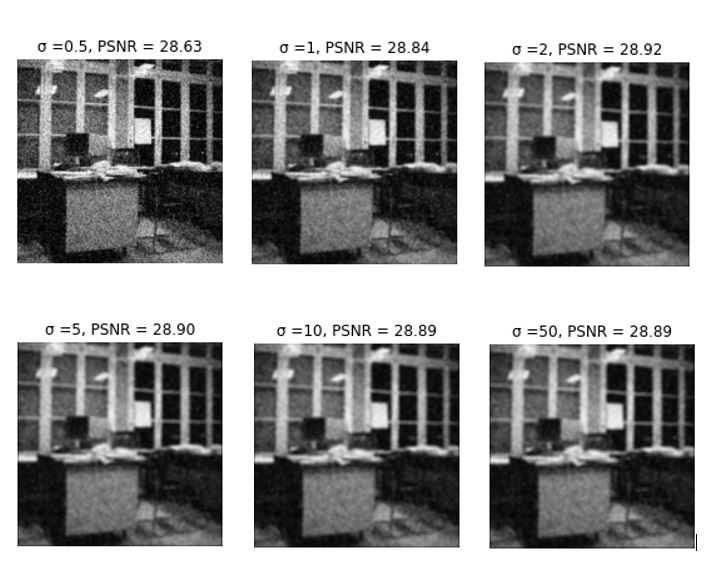
\includegraphics[scale=0.75]{./images/Gaussian_Blur}
\caption{Gaussian smoothing with different $\sigma$ values.}
\label{fig:example}
\end{center}
\end{figure}


\subsection{Denoising by Isotropic Linear Diffusion}

Keeping the diffusivity constant as 1, diffusion time is varied as $t = \{1, 5, 10, 30, 100\}$. Image is discretized with padding to compensate the Dirichlet boundary conditions applied at the boundary of the image which is defined by its size.

With Fig. 2, It could be construed that, Noise is reduced for increasing diffusion time till a point, after which the image becomes blurry, removing all necessary details and edge information.
From Fig. 1 and Fig. 2, It can be inferred that Gaussian smoothing and Isotopic linear diffusion tend to blur the image beyond a threshold thereby removing useful information of the images like edges along with the noise. Yet owing to the numerical approximation, discrepancies could be observed on proving them equal with the noisy image, hence this fact is verified to be false.
\begin{figure}[!htbp]
\begin{center}
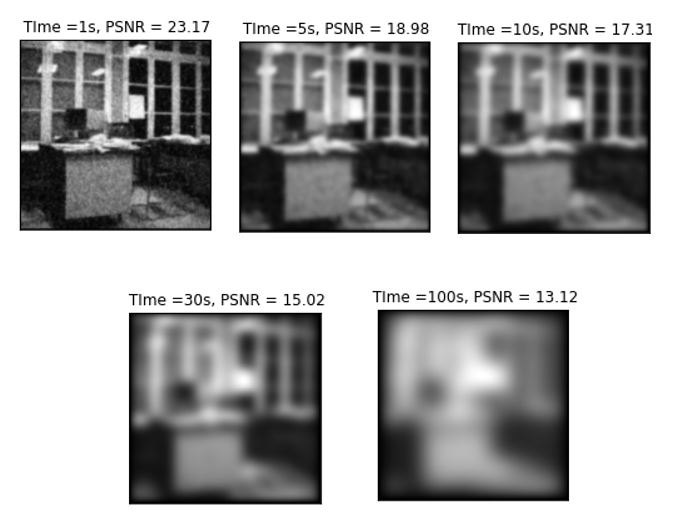
\includegraphics[scale=0.75]{./images/IsotropicLinearDiffusion}
\caption{Isotopic linear diffusion smoothing with different diffusion time values.}
\label{fig:example}
\end{center}
\end{figure}

From Fig. 3, It is clearly evident that image becomes more blurry for increasing diffusion time at a constant diffusivity, as even at edges the gray scale values are diffused uniformly leading to dispersion of details in the image.




\begin{figure}[!htbp]
\begin{center}
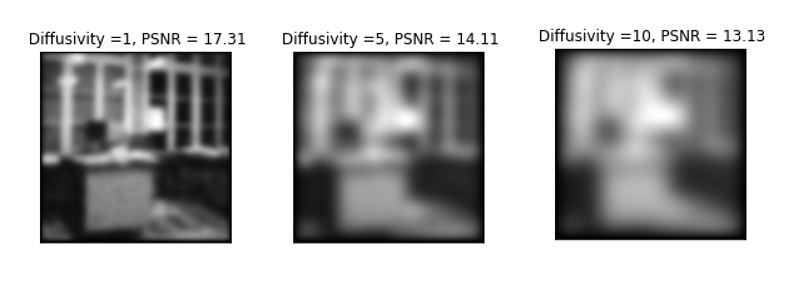
\includegraphics[scale=0.75]{./images/IsotropicLinear_ChangingD}
\caption{Isotopic linear diffusion smoothing with different diffusivity values.}
\label{fig:example}
\end{center}
\end{figure}

%------------------------------------------------------------------------------
\subsection{Denoising by Isotropic Non-Linear Diffusion}
Isotropic non-linear diffusion equation is solved with initial condition as noisy office image and boundary conditions are Dirichlet, it can be observed form Fig. 4 that noise is reduced till t= 10s, then for increasing time, entire image is smoothed along with noise, resulting in adverse effects.

\begin{figure}[!htbp]
\begin{center}
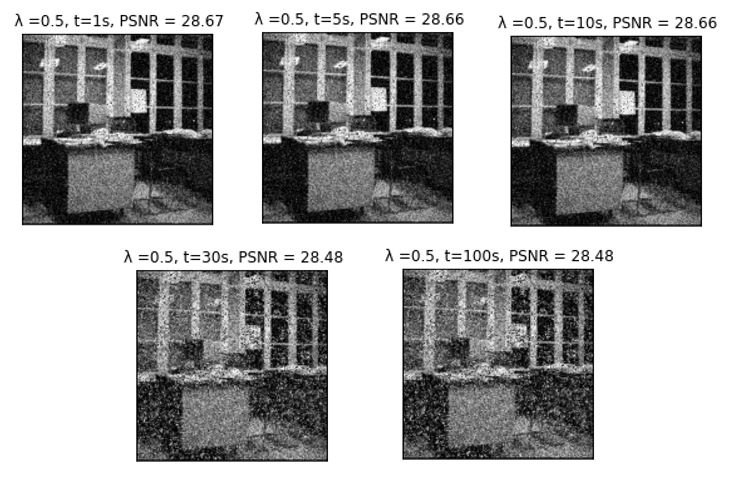
\includegraphics[scale=0.75]{./images/IsotropicNonLinear_ChangedTime}
\caption{Isotopic Non-linear diffusion smoothing with different diffusion time values.}
\label{fig:example}
\end{center}
\end{figure}

On computing the diffusivity of noiseless image with $\lambda$ = 0.5, as per Fig.5, it's evident that the diffusivity has lessened at the edges resulting in higher gray pixel values at the edges, hence the details are preserved as the name "edge preserving" diffusion.

\begin{figure}[!htbp]
\begin{center}
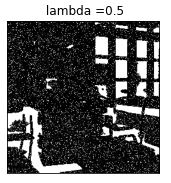
\includegraphics[scale=1]{./images/Non_linear_Diffusivity}
\caption{Diffusivity as a gray-scale image.}
\label{fig:example}
\end{center}
\end{figure}

Comparison of Fig.2 and Fig. 4 throws light on the fact that non-linear diffusion preserves edges better than linear diffusion.

Finally on setting higher contrast values for a constant diffusion time, the concentration of the edges seems to collide with the normal regions resulting in a degraded performance.

\begin{figure}[!htbp]
\begin{center}
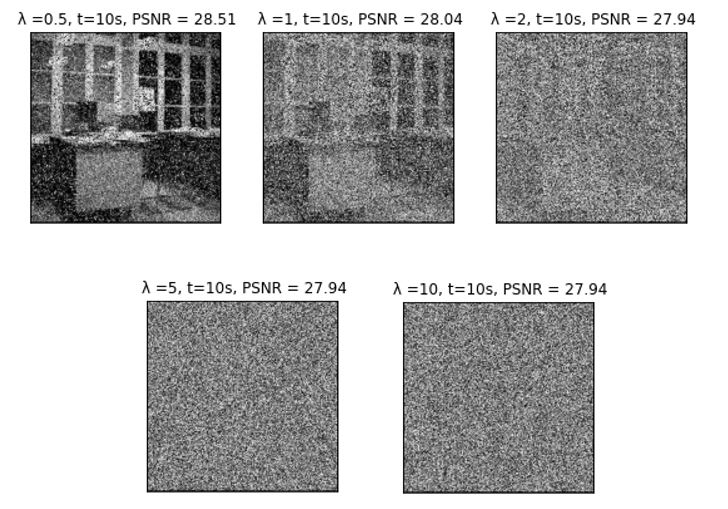
\includegraphics[scale=0.75]{./images/Non_linear_varingLambda}
\caption{Isotopic Non-linear diffusion smoothing with different  $\lambda$ values.}
\label{fig:example}
\end{center}
\end{figure}


\section{Conclusion}
Advancements in image denoising has been on forefront since the arrival of cameras in 1800's, This paper explores the basic image denoising techniques, among which non-linear diffusion smoothing works better at preserving edges than Gaussian/linear diffusion smoothing, while the later can be employed as a first step in any image processing technique to process a image with a lot of noise. Careful consideration of parameters like diffusion time, diffusivity coefficient and the method for solving the diffusion equation can improve the denoising process in whole.

%----------------------------------------------------------------------------
\section*{Acknowledgment}

Thanks to Dr.Kartheek Popuri and Dr.Hamilton Matthew for providing this assignment for evaluating my skills for graduate education.

%------------------------------------------------------------------------------
\section*{Image Credits}

{\small
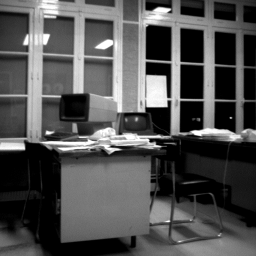
\includegraphics[height=2em]{./images/office}
  Office Image\\
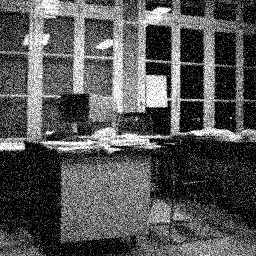
\includegraphics[height=2em]{./images/office_noisy}
  Noisy Office Image
}

%------------------------------------------------------------------------------

\bibliographystyle{unsrt}
\bibliography{article}

\end{document}
%------------------------------------------------------------------------------
